%!TEX root = ../TAMUTemplate.tex
%%%%%%%%%%%%%%%%%%%%%%%%%%%%%%%%%%%%%%%%%%%%%%%%%%%
%
%  New template code for TAMU Theses and Dissertations starting Fall 2016.
%
%  Author: Sean Zachary Roberson
%	 Version 3.16.09
%  Last updated 9/12/2016
%
%%%%%%%%%%%%%%%%%%%%%%%%%%%%%%%%%%%%%%%%%%%%%%%%%%%

%%%%%%%%%%%%%%%%%%%%%%%%%%%%%%%%%%%%%%%%%%%%%%%%%%%%%%%%%%%%%%%%%%%%%%%
%%%                           SECTION IV
%%%%%%%%%%%%%%%%%%%%%%%%%%%%%%%%%%%%%%%%%%%%%%%%%%%%%%%%%%%%%%%%%%%%%%


\chapter{\uppercase {Analysis Strategy}}

This search for the Higgs boson uses a final state with one well reconstructed (tight) lepton, two or more jets, and some \ETslash, coming exclusively from the unreconstructed neutrino. The search is broken up into six channel by lepton flavor (electron or muon) and the number of jets (two, three, and four or more). Previous searches, like the high mass analysis 

\section{Data \& MC Samples}

As mentioned previously, this analysis makes use of the full 2012 dataset of 8\tev data. Table~\ref{tab:dataSamples} shows the data samples used for this analysis, which corresponds to $\sim$19.2\fbinv. The luminosities listed in the table are associated with a 4.4\% uncertainty as specified in~\cite{CMS-PAS-LUM-12-001} and were collected using the HF luminosity measurements.

\begin{table}[hbtp]\footnotesize
\centering
\begin{tabular}{|l|c|r|}
\hline\hline
 Dataset & Run Range & Integrated Luminosity \\
\hline
/SingleMu/Run2012A-13Jul2012-v1/AOD & 190645-196531 & 0.809$\fbinv$ \\
/SingleMu/Run2012A-recover-06Aug2012-v1/AOD & 190782-190949 & 0.082$\fbinv$ \\
/SingleMu/Run2012B-13Jul2012-v1/AOD & 193834-196531 & 4.383$\fbinv$ \\
/SingleMu/Run2012C-24Aug2012-v1/AOD & 198022-198523 & 0.489$\fbinv$ \\
/SingleMu/Run2012C-PromptReco-v2/AOD & 194631-203002 & 6.285$\fbinv$ \\
/SingleMu/Run2012D-PromptReco-v1/AOD & 194480-208686 & 7.231$\fbinv$ \\
{\bf Total SingleMu} & {\bf 190645--208686} & {\bf 19.279$\fbinv$} \\
\hline
/SingleElectron/Run2012A-13Jul2012-v1/AOD & 190645-196531 & 0.809$\fbinv$ \\
/SingleElectron/Run2012A-recover-06Aug2012-v1/AOD & 190782-190949 & 0.082$\fbinv$ \\
/SingleElectron/Run2012B-13Jul2012-v1/AOD & 193834-196531 & 4.336$\fbinv$ \\
/SingleElectron/Run2012C-24Aug2012-v1/AOD & 198022-198523 & 0.489$\fbinv$ \\
/SingleElectron/Run2012C-PromptReco-v2/AOD & 194631-203002 & 6.194$\fbinv$ \\
/SingleElectron/Run2012D-PromptReco-v1/AOD & 194480-208686 & 7.238$\fbinv$\\
{\bf Total SingleElectron} & {\bf 190645--208686} & {\bf 19.148$\fbinv$} \\
\hline

\hline\hline
\end{tabular}
\caption{The datasets analyzed for this analysis.}
\label{tab:dataSamples}
\end{table}

The backgrounds were modeled by MC samples generated with \textsc{MadGraph}~\cite{Alwall:2014hca} and \textsc{pythia6}~\cite{1126-6708-2006-05-026}. 
The signal MC samples were also generated by \textsc{pythia6}.
Tables~\ref{tab:bkgSamples} and~\ref{tab:SignalSamples} show the background and signal MC samples used.
Rather than relying on MC for the QCD background sample, a data-driven sample was created by using the same trigger requirements as the data, but removing the isolation requirement for the lepton and inverting the lepton particle flow isolation cut during selection.
This process provides a completely orthogonal sample of QCD events from data.
The normalization of this background is found by doing a two component fit to the data, allowing only the W+jets and QCD fractions to float.

\begin{table}[hbtp]\footnotesize
\centering
\begin{tabular}{|c|p{0.65\textwidth}|r|}
\hline\hline
Sample & Dataset & Cross Sect. \\
\hline
W+jets & /WJetsToLNu\_TuneZ2Star\_8TeV-madgraph-tarball/Summer12\_DR53X-PU\_S10\_START53\_V7A-v1/AODSIM\newline/WJetsToLNu\_TuneZ2Star\_8TeV-madgraph-tarball/Summer12\_DR53X-PU\_S10\_START53\_V7A-v2/AODSIM & 37509 pb\\ \hline
$\ttbar$ & /TTJets\_MassiveBinDECAY\_TuneZ2star\_8TeV-madgraph-tauola/Summer12\_DR53X-PU\_S10\_START53\_V7A-v1/AODSIM & 225.197 pb\\\hline
Z+jets & /DYJetsToLL\_M-50\_TuneZ2Star\_8TeV-madgraph-tarball/Summer12\_DR53X-PU\_S10\_START53\_V7A-v1/AODSIM & 3387.6 pb\\\hline
WW & /WW\_TuneZ2star\_8TeV\_pythia6\_tauola/Summer12\_DR53X-PU\_S10\_START53\_V7A-v1/AODSIM& 54.838 pb\\\hline
WZ & /WZ\_TuneZ2star\_8TeV\_pythia6\_tauola/Summer12\_DR53X-PU\_S10\_START53\_V7A-v1/AODSIM& 33.21 pb\\\hline
ZZ & /ZZ\_TuneZ2star\_8TeV\_pythia6\_tauola/Summer12\_DR53X-PU\_S10\_START53\_V7A-v1/AODSIM& 17.654 pb\\\hline
Single \cPqt & & \\
t-Channel & /T\_t-channel\_TuneZ2star\_8TeV-powheg-tauola/Summer12\_DR53X-PU\_S10\_START53\_V7A-v1/AODSIM& 56.4 pb\\
tW-Channel & /T\_tW-channel-DR\_TuneZ2star\_8TeV-powheg-tauola/Summer12\_DR53X-PU\_S10\_START53\_V7A-v1/AODSIM& 11.1 pb\\
s-Channel & /T\_s-channel\_TuneZ2star\_8TeV-powheg-tauola/Summer12\_DR53X-PU\_S10\_START53\_V7A-v1/AODSIM& 3.79 pb\\\hline
Single \cPaqt & & \\
SingleTbar t-Channel & /Tbar\_t-channel\_TuneZ2star\_8TeV-powheg-tauola/Summer12\_DR53X-PU\_S10\_START53\_V7A-v1/AODSIM& 30.7 pb\\
SingleTbar tW-Channel & /Tbar\_tW-channel-DR\_TuneZ2star\_8TeV-powheg-tauola/Summer12\_DR53X-PU\_S10\_START53\_V7A-v1/AODSIM& 11.1 pb\\
SingleTbar s-Channel & /Tbar\_s-channel\_TuneZ2star\_8TeV-powheg-tauola/Summer12\_DR53X-PU\_S10\_START53\_V7A-v1/AODSIM& 1.76 pb\\\hline
QCD & & \\
Electron & See table~\ref{tab:dataSamples} for a list of SingleElectron datasets & N/A \\
Muon & See table~\ref{tab:dataSamples} for a list of SingleMu datasets & N/A \\

\hline\hline
\end{tabular}
\caption{List of background MC datasets and cross sections used for normalization.}
\label{tab:bkgSamples}
\end{table}

Several corrections are made to the MC before use.
When MC is made it is generated with an assumption of what the pileup (PU) distribution will look like in data.
However, this guess is rarely accurate and the MC must be reweighted such that the correct PU distribution is reflected in the MC.
The weights are created by using special measurements in CMS which measure the true number of PU interactions in data and dividing this histogram by the number of true interactions coming from MC.
This provides the weights as a function of the true number of proton-proton interactions.
Each MC sample has this weight applied.

\begin{table}[hbtp]\footnotesize
\centering
\begin{tabular}{|c|p{0.65\textwidth}|r|r|}
\hline\hline
Sample Name & Dataset & Cross Sect. & BR\\  \hline
g-g Higgs & /LQ-ggh125\_BIG\_SIM\_ggH125\_part1/aperloff-LQ-ggh125\_AODSIM\_Summer12\_START53\_V7E-768a14b04b0ac2af0d20e6783fbdb759/USER & 19.27pb & 0.0947 \\
  & /LQ-ggh125\_BIG\_GEN\_part2/aperloff-LQ-ggh125\_BIG\_RECO\_part2-33e909ff21293ad9fa8564de2959fe54/USER & 19.27pb & 0.0947\\
  & /LQ-ggh125\_BIG\_GEN\_part3/aperloff-LQ-ggh125\_BIG\_RECO\_part3-33e909ff21293ad9fa8564de2959fe54/USER & 19.27pb & 0.0947\\
  & /LQ-ggh125\_Part6\_SIM/goodell-LQ-qqh125\_RECO\_Part6-33e909ff21293ad9fa8564de2959fe54/USER & 19.27pb & 0.0947\\
  & /LQ-ggh125\_Part7\_SIM/goodell-LQ-qqh125\_RECO\_Part7-33e909ff21293ad9fa8564de2959fe54/USER & 19.27pb & 0.0947\\
  & /LQ-ggh125\_Part8\_GENSIM/goodell-LQ-ggh125\_Part8\_RECO-33e909ff21293ad9fa8564de2959fe54/USER & 19.27pb & 0.0947\\ \hline
VBF Higgs & /LQ-vbf125\_GENSIM/ajkumar-LQ-qqh125\_AODSIM\_Summer12\_{\newline}START53\_V7A-c8f8ed334db8a7d6f56c62266b1dfa5b/USER & 1.578pb & 0.0947\\
Ass. Prod. Higgs & WH\_ZH\_TTH\_HToWW\_M-125\_8TeV-pythia6/Summer12\_DR53X-PU\_S10\_START53\_V7A-v1/AODSIM & 1.249pb & 0.215\\ \hline
\multicolumn{4}{c}{Non signal Higgs Production} \\ \hline
Ass. Prod. Higgs & WH\_ZH\_TTH\_HToZZ\_M-125\_8TeV-pythia6/Summer12\_DR53X-PU\_S10\_START53\_V7A-v1/AODSIM & 1.249pb & 0.0264\\
  & WH\_WToLNu\_HToBB\_M-125\_8TeV-powheg-herwigpp/Summer12\_DR53X-PU\_S10\_START53\_V7A-v1/AODSIM & 0.7046pb & 0.1879\\
  & /TTH\_HToBB\_M-125\_8TeV-pythia6/Summer12\_DR53X-PU\_S10\_START53\_V7A-v1/AODSIM & 0.1293pb & 0.577\\
\hline\hline
\end{tabular}
\caption{List of Signal datasets and cross sections}
\label{tab:SignalSamples}
\end{table}

There are additional MC corrections that go beyond the scope of this proposal, but which are nevertheless used in the analysis.
The jet energy corrections and jet energy resolution scale factors make sure that the energy and resolution of the jets in MC matches those used in data and that the overall scale is correct.
The $\ETslash_{\varphi}$ corrections remove a modulation in the \ETslash 4-momentum, which appears as a function of the number of proton-proton interactions.
There is a reweighting of the events to correct the b-tag discriminant distributions and a reweighting to correct the \pt distributions of the \ttbar MC being used.
We also correct for a mis-modeling of the $\cos\left(\theta_{l}\right)$ angular variable and to accurately model QCD in the isolated lepton region even when the data-driven QCD sample is taken from the anti-isolated lepton region.

\section{Signal and Control Regions}

This analysis is searching for a Higgs boson which decays to two W bosons, one of which decays hadronically and the other which decays leptonically.
Therefore the signal region for the search includes one tight lepton, at least 25\gev of \ETslash, and at least two jets.
The vertex, jets, and lepton requirements all meet the object requirements as defined by CMS.
The minimum electron (muon) \pt was set to 30\gev (25\gev) and the minimum jet \pt was set to 25\gev, except for the leading jet, which is required to have a \ptgt{30\gev}.
As the hadronic W decay will have at least two jets, that is the minimum number of jets needed to make it into the signal region, but we do not veto on additional jets which might come from ISR or FSR.
The \ETslash requirement is there because of the neutrino from the leptonic decay of the W, but is set to a value on the higher side to remove as much QCD as possible without cutting out too much signal.
Additionally, a b-tag veto is implemented for two reasons.
The first is because hadronically decaying W only rarely decay to b-jets, but the \ttbar background includes at least two b-jets in its final state.
The second reason is to keep this analysis orthogonal to the VH(H$\rightarrow${bb}) search~\cite{PhysRevD.89.012003}.
Table~\ref{tab:FinalYields} shows the expected event yields in the signal region.

Two main control regions are defined based on the aforementioned signal selection criteria.
The first includes all of the same cuts as the signal region, but only one jets.
This region is used for the normalization of the data-driven QCD sample.
A second control region requires there to be exactly 1 b-jet.
This region is used to check the volunteer signal contribution and the efficacy of the b-tag veto.

\begin{table}[htbp]
  \centering
  \noindent
  \small
    \begin{tabular}{|l|c|c|c|} \hline \hline
Process & $==$ 2 & $==$ 3 &  $\geq$4 \\ \hline
Diboson  & 39026.22 $\pm$ 197.55 & 12612.58 $\pm$ 112.31 & 3485.46 $\pm$ 59.04 \\
$W$+jets  & 3271138.31 $\pm$ 1808.63 & 726384.44 $\pm$ 852.28 & 187723.52 $\pm$ 433.27 \\
$Z$+jets  & 272583.99 $\pm$ 522.10 & 69588.32 $\pm$  263.80 & 19937.11 $\pm$ 141.20 \\
$t\bar{t}$  & 20005.51 $\pm$ 141.44 & 24748.61 $\pm$ 157.32 & 27686.99 $\pm$ 166.39 \\
Single $t$ & 16318.38 $\pm$ 127.74 & 7096.2 $\pm$ 84.24 & 3036.83 $\pm$ 55.11 \\
Multi-Jet  & 450503.85 $\pm$ 671.20 & 119248.8 $\pm$ 345.32 & 33681.6 $\pm$ 183.53 \\ \hline
Tot Bkg & 4069576.26 $\pm$ 2017.32 & 959678.95 $\pm$ 979.63 & 275551.51 $\pm$ 524.93 \\\hline \hline
ggH, H$\rightarrow$WW $M_{H}=125$  & 548.49 $\pm$ 23.42 & 210.97 $\pm$ 14.52 & 79.87 $\pm$ 8.94 \\
qqH, H$\rightarrow$WW $M_{H}=125$  & 106.34 $\pm$ 10.31 & 52.53 $\pm$ 7.25 & 17.47 $\pm$ 4.18\\
WH\_ZH\_TTH, H$\rightarrow$WW $M_{H}125$ & 124.51 $\pm$ 11.16 & 77.97 $\pm$ 8.83 & 42.95 $\pm$ 6.55\\
WH\_ZH\_TTH, H$\rightarrow$ZZ $M_{H}125$ & 8.27 $\pm$ 2.88 & 4.4 $\pm$ 2.10 & 2.25 $\pm$ 1.50\\
WH, H$\rightarrow$b$\bar{b}$ $M_{H}125$ & 40.2 $\pm$ 6.34 & 12.63 $\pm$ 3.55 & 3.39 $\pm$ 1.84\\
TTH, H$\rightarrow$b$\bar{b}$ $M_{H}=125$ & 0.53 $\pm$ 0.73 & 1.14 $\pm$ 1.07 & 3.14 $\pm$ 1.77 \\ \hline
Total Signal & 828.33 $\pm$ 28.78 & 359.64 $\pm$ 18.96 & 149.07 $\pm$ 12.21 \\ \hline
    \end{tabular}
    \caption{Expected event yield in the signal region after combining the lepton channels.}
    \label{tab:FinalYields}
\end{table}

\section{Matrix Elements}

Table~\ref{tab:FinalYields} clearly shows that the total signal, in every channel, is smaller than even the statistical uncertainty of the background.
A cut and count experiment will not lead to any significant results.
The previous \HWWlnujj analyses have performed a fit to sensitive distributions like the 4-body mass, the mass of the two jet plus lepton plus \ETslash system.
However, this approach only includes a small amount of information available, leaving out additional sensitive kinematic distributions.
It is also felt that a BDT analysis using only kinematic variable would be sub-optimal because shallow classifiers are not robust against non-linear correlations and are only as good as the input variables.

Instead, this analysis uses a matrix element method (MEM), which starts from the differential cross section calculation from quantum field theory to classify how likely and event is to come from a given process~\cite{Canelli2003,Dong2008}.
The probability $P\left(x;\alpha\right)=P_{evt}$ of a signal is proportional to the differential production cross section, where $\alpha$ is the parameter we wish to measure and x is a set of physical variables.
This is true if the detector resolution is sufficiently small and the beam energies are well known, as it is in the case of CMS.
In general the differential cross section can be written as~\cite{Olive:2016xmw}:
\begin{equation}\label{eq:differential_production_cross_section}
d\sigma=\frac{\left(2\pi\right)^{4}|\mathcal{M}|^{2}}{4\sqrt{\left(q_{1}\cdot{q_{2}}\right)^{2}-m_{q_{1}}^{2}m_{q_{2}}^{2}}}d\Phi_{n}\left(q_{1}+q_{2};p_{1},...,p_{n}\right)
\end{equation}
where $|\mathcal{M}|$ is the Lorentz invariant matrix element (ME); $q_{1}$, $q_{2}$ and $m_{1}$, $m_{2}$ are the 4-momenta and masses of the incident particles; $p_{i}$ are the 4-momenta of the final state particles; and $d\Phi_{n}$ is the n-body phase space.
The phase space term is written as:
\begin{equation}
d\Phi_{n}\left(q_{1}+q_{2};p_{1},...,p_{n}\right)=\delta^{4}\left(q_{1}+q_{2}-\sum_{i=1}^{n}p_{i}\right)\prod_{i=1}^{n}\frac{d^{3}p_{i}}{\left(2\pi\right)^{3}2E_{i}}
\end{equation}
After accounting for unmeasured or mis-measured particles and normalizing to the total cross section to form an event probability, equation~\ref{eq:differential_production_cross_section} becomes:
\begin{equation}
P(x;\alpha)=\frac{1}{\sigma}\int2\pi^{4}|\mathcal{M}|^{2}\frac{f\left(x_{1}\right)}{|E_{q_{1}}|}\frac{f\left(x_{2}\right)}{|E_{q_{2}}|}W\left(y,x\right)d\Phi_{4}dE_{q_{1}}dE_{q_{2}}
\end{equation}
where $f\left(x_{i}\right)$ are the PDFs, $x_{i}=E_{q_{i}}/E_{beam}$ is the fraction of the proton momentum carried by the incident parton $i$, and $W\left(y,x\right)$ is the transfer function mapping measured jet energies $x$ to the parton energies $y$ (accounts for the jet resolution of CMS).

Fifteen probabilities $P(x;\alpha)$, corresponding to the leading order diagrams of the major background and signal processes, are computed for each event. 
This computation is by far the most time consuming aspect of this analysis, consuming $\sim$12 million CPU hours.
The information contained in these 15 probabilities must be combined in order to discriminate signal from background.

\section{Signal Extraction}

In order to combine the complimentary information from the kinematic variables and the MEs, with the purpose of discriminating a Higgs event from a background event, we used several Boosted Decision Trees (BDTs).
An initial BDT was computed which combined the information from 15 of the computed MEs.\footnote{A BDT was used rather than combining the ME into a likelihood as in the Matrix Element Likelihood Analysis (MELA) used by H$\rightarrow$ZZ$\rightarrow$4l or using some basic ratios of signal over background probabilities as was done by CDF.}
This gives a less discriminating shallow network the ability to create a better performing network because the inputs are already non-linear variables.
The output of this BDT, along with several carefully selected kinematic variables, is then used as the input to a new BDT in order to combine all of this complimentary information.
While it may seem that the MEs should encode all of the event information perfectly, only the leading MEs were used and the permutations of the jets and partons degrades the discrimination power of the MEs.
The combined BDT has more discrimination power than either the MEs or the kinematic variables alone. 

A distribution of the BDT discriminant is produced for every signal, background, and data sample and then passed to the RooStats-based Higgs Combine Tool~\cite{CombineToolTwiki} to compute limits on the Higgs signal strength.
Given that this analysis has a relatively high number of events in the expected yields we make use of the asymptotic method\footnote{If there had been a lower number of expected events we may have needed to use the full frequentist method rather than the asymptotic method.} for limit setting along with the CL\textsubscript{s} test statistic~\cite{Read:2002hq}.
Using an Asimov dataset an expected 95\% upper confidence level is obtained and shown in figure~\ref{fig:limits} (left).

\section{Systematics}

Given that this is a shape analysis, it is important to consider systematic uncertainties that may change the expected yields (rate changes), the shape of the discriminating variable, or both.
This analysis considers all three of these, but decouples the rate and shape changes during limit setting.
Table~\ref{tab:ListOfSystematics} summarizes all of the systematic uncertainties considered for this analysis.
Changes to the limits greater than 1\% come from the scheme used to reweight the $\eta$ distribution in the QCD sample, the jet energy scale, the $\cos\left(\theta_{l}\right)$ weights, and the lepton efficiency uncertainty.
There will be much more detail on each of the systematics in the thesis.

\begin{table}[htbp]
  \centering
  \noindent
  \small
    \captionsetup{width=.85\textwidth}
    \caption*{Systematic Uncertainties for H$\rightarrow$WW$\rightarrow$l$\nu$jj Analysis}
    \begin{tabular}{|l|c|c|c|} \hline
Uncertainty & Rate (Y/N) 2 & Shape (Y/N) & Comments \\ \hline
$Q^{2}$ Scaling & Y & Y & W+jets MC only \\ \hline
ME/PS Matching & Y & Y & W+jets MC only \\ \hline
Background xSec & Y & N & All background samples \\  \hline
Signal xSec & Y & N & All signal MC samples \\  \hline
Luminosity & Y & N & All samples \\  \hline
MC Pileup reweighting & Y & N & All MC samples \\  \hline
Trigger Efficiency & Y & N &  All MC samples\\  \hline
Lepton Selection Efficiency & Y & N & All MC samples\\  \hline
JES Uncertainties & Y & Y & All MC samples \\  \hline
Met Uncertainty & Y & N & All samples\\  \hline
CSV Reshaping & Y & N &  All MC samples\\  \hline
Top Pt-reweighting & Y & Y &  TTbar MC only\\  \hline
QCD $\eta$ Weight & Y & Y & QCD shape, W+jets and QCD rate \\ \hline
$\cos\left(\theta_{l}\right)$ Weight & N & Y & W+jets MC only \\ \hline
    \end{tabular}
    \caption{List of all systematic uncertainties applied in analysis, whether that uncertainty has a rate or shape component to it, and which samples is is applied to.}
    \label{tab:ListOfSystematics}
\end{table}

\section{Limits \& Plans}

Final limits, including all systematics are calculated again using the Higgs Combine Tool.
Figure~\ref{fig:limits} (right) shows the expected limits with the systematic uncertainties included.
The final product will be a similar plot including the observed limits.
This will be presented in the thesis and during the final exam.

\begin{figure}[!hbt]
	\centering
	\begin{subfigure}[t]{0.46\textwidth}
		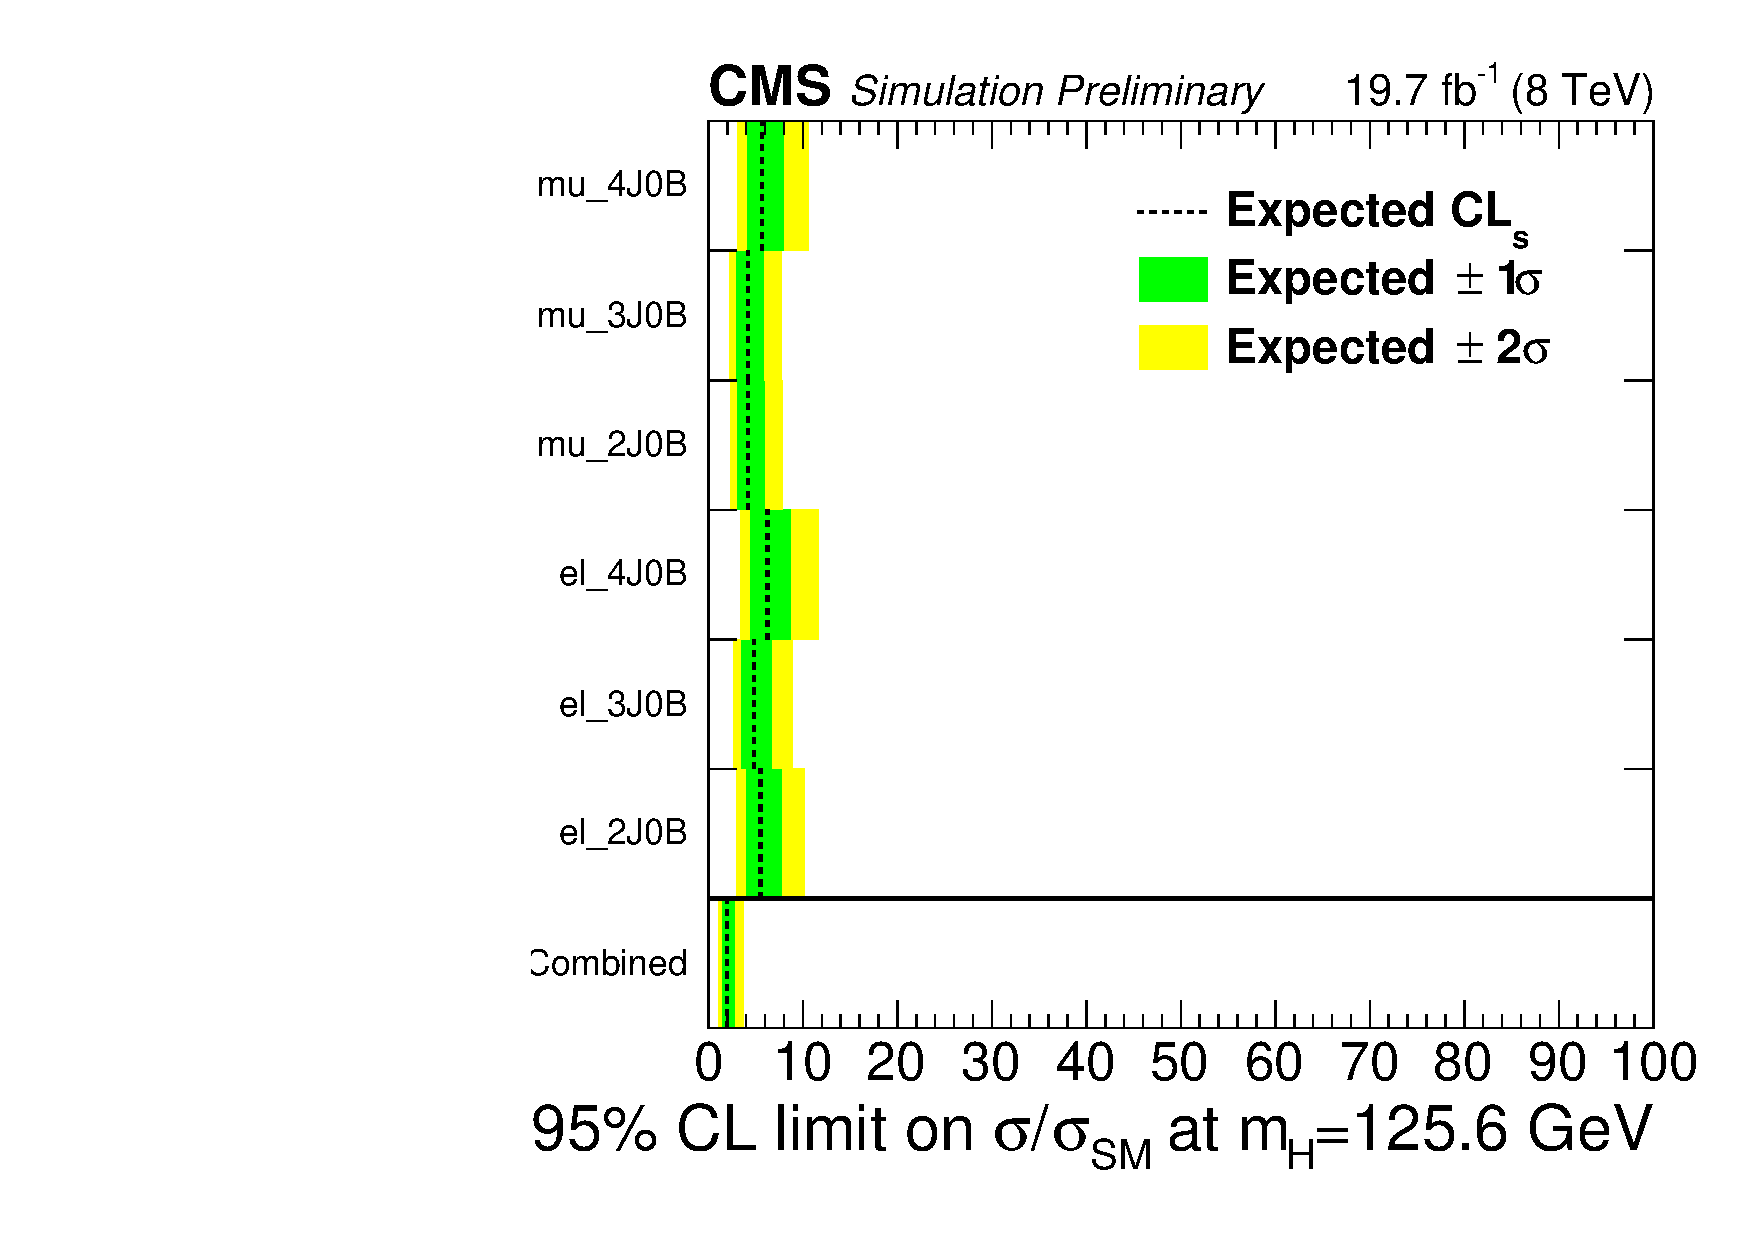
\includegraphics[width=\textwidth]{\figpath/Chapter4/2015_08_01_combinedSM_KinMEBDT_StatsOnly.pdf}
		\label{fig:limits_stats_only}
	\end{subfigure}
	\begin{subfigure}[t]{0.46\textwidth}
		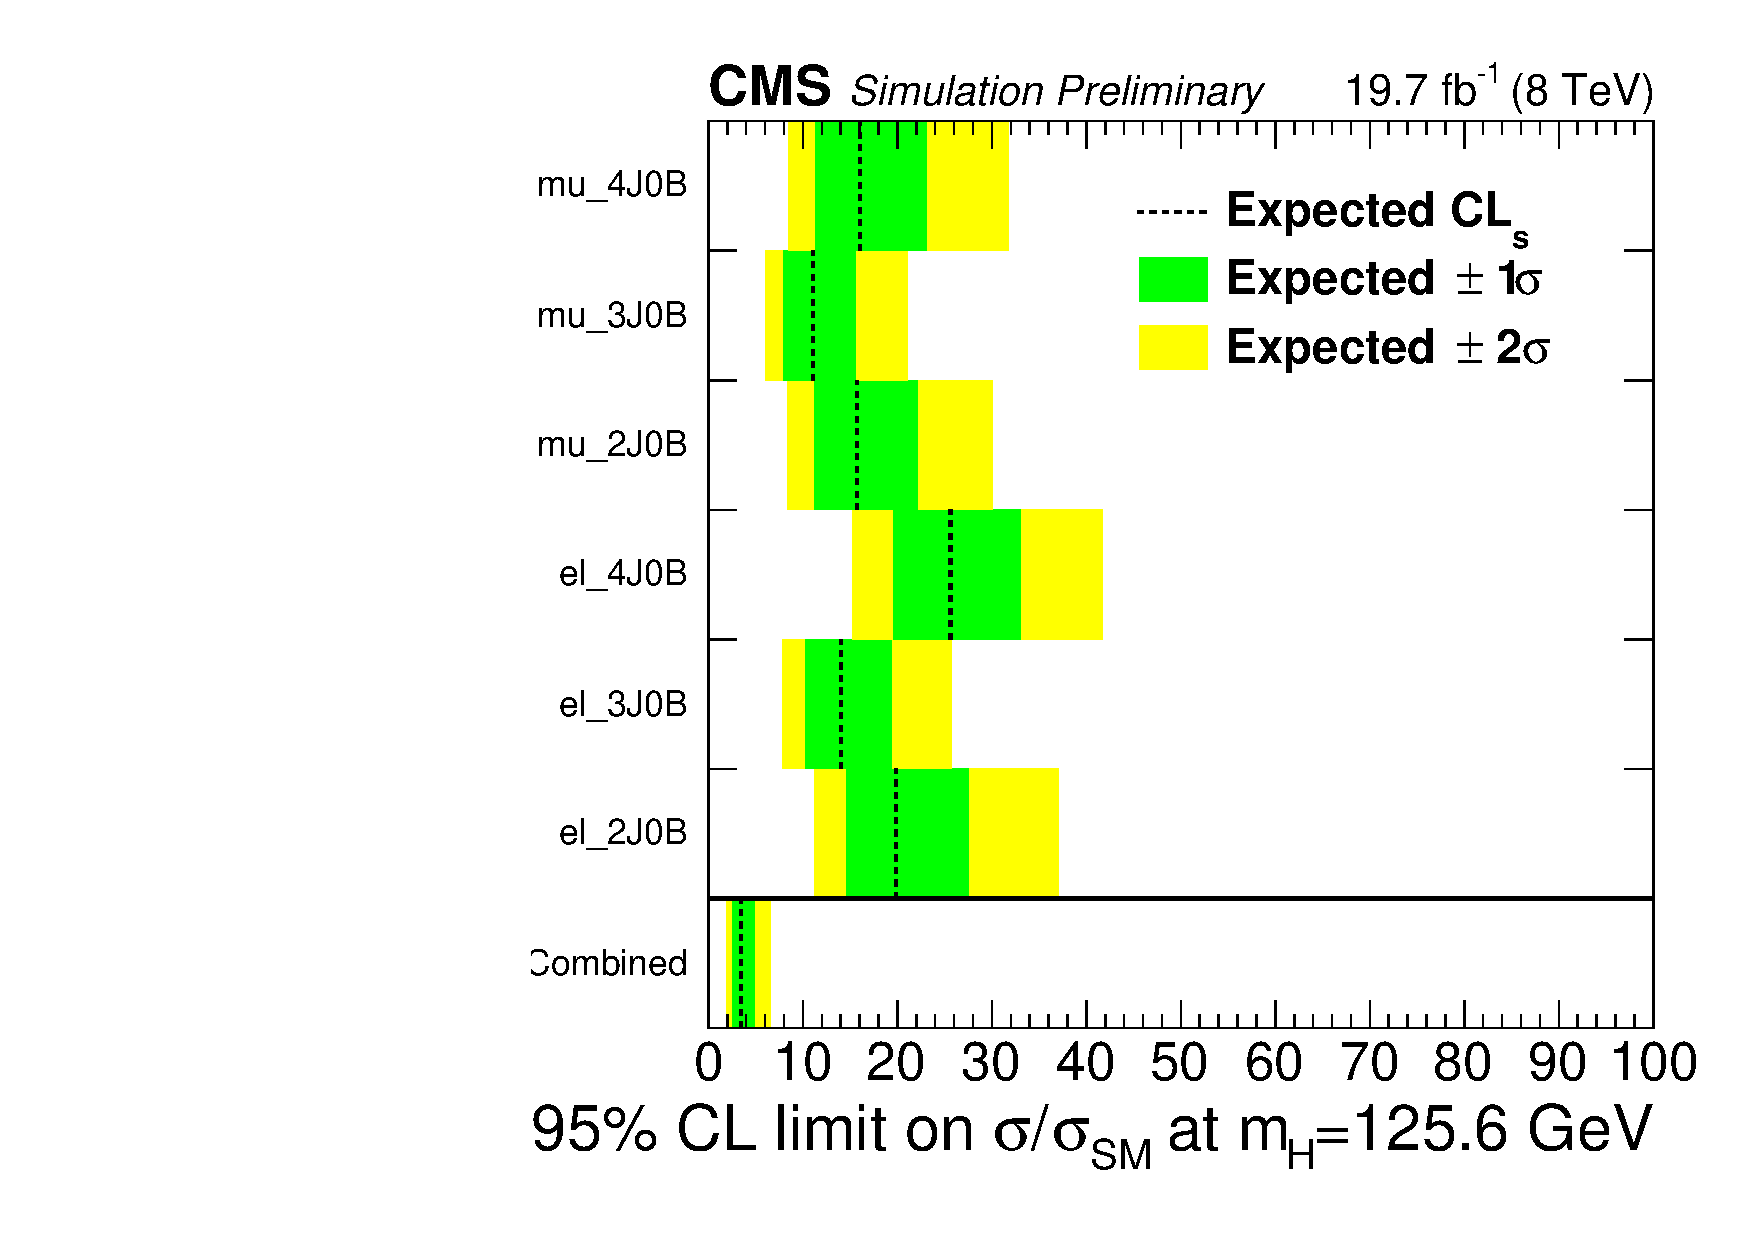
\includegraphics[width=\textwidth]{\figpath/Chapter4/2015_08_01_combinedSM_KinMEBDT.pdf}
		\label{fig:limits_with_sys}
	\end{subfigure}
	\caption{Expected 95\% upper confidence level on the Higgs signal strength (left) without including systematic uncertainties and (right) with systematic uncertainties included. The median combined limit is found to be 2.01 without systematics and 3.48 with them.}
	\label{fig:limits}
\end{figure}
